\documentclass[12pt,letterpaper]{article}\usepackage[]{graphicx}\usepackage[]{color}
%% maxwidth is the original width if it is less than linewidth
%% otherwise use linewidth (to make sure the graphics do not exceed the margin)
\makeatletter
\def\maxwidth{ %
  \ifdim\Gin@nat@width>\linewidth
    \linewidth
  \else
    \Gin@nat@width
  \fi
}
\makeatother

\definecolor{fgcolor}{rgb}{0.345, 0.345, 0.345}
\newcommand{\hlnum}[1]{\textcolor[rgb]{0.686,0.059,0.569}{#1}}%
\newcommand{\hlstr}[1]{\textcolor[rgb]{0.192,0.494,0.8}{#1}}%
\newcommand{\hlcom}[1]{\textcolor[rgb]{0.678,0.584,0.686}{\textit{#1}}}%
\newcommand{\hlopt}[1]{\textcolor[rgb]{0,0,0}{#1}}%
\newcommand{\hlstd}[1]{\textcolor[rgb]{0.345,0.345,0.345}{#1}}%
\newcommand{\hlkwa}[1]{\textcolor[rgb]{0.161,0.373,0.58}{\textbf{#1}}}%
\newcommand{\hlkwb}[1]{\textcolor[rgb]{0.69,0.353,0.396}{#1}}%
\newcommand{\hlkwc}[1]{\textcolor[rgb]{0.333,0.667,0.333}{#1}}%
\newcommand{\hlkwd}[1]{\textcolor[rgb]{0.737,0.353,0.396}{\textbf{#1}}}%

\usepackage{framed}
\makeatletter
\newenvironment{kframe}{%
 \def\at@end@of@kframe{}%
 \ifinner\ifhmode%
  \def\at@end@of@kframe{\end{minipage}}%
  \begin{minipage}{\columnwidth}%
 \fi\fi%
 \def\FrameCommand##1{\hskip\@totalleftmargin \hskip-\fboxsep
 \colorbox{shadecolor}{##1}\hskip-\fboxsep
     % There is no \\@totalrightmargin, so:
     \hskip-\linewidth \hskip-\@totalleftmargin \hskip\columnwidth}%
 \MakeFramed {\advance\hsize-\width
   \@totalleftmargin\z@ \linewidth\hsize
   \@setminipage}}%
 {\par\unskip\endMakeFramed%
 \at@end@of@kframe}
\makeatother

\definecolor{shadecolor}{rgb}{.97, .97, .97}
\definecolor{messagecolor}{rgb}{0, 0, 0}
\definecolor{warningcolor}{rgb}{1, 0, 1}
\definecolor{errorcolor}{rgb}{1, 0, 0}
\newenvironment{knitrout}{}{} % an empty environment to be redefined in TeX

\usepackage{alltt}
\usepackage[utf8]{inputenc}
\usepackage[margin=.7in]{geometry}
\usepackage{graphicx}
\usepackage{titling}
\usepackage{amsmath}
\usepackage{amsfonts}
\usepackage{amssymb}
\renewcommand{\theenumiv}{\arabic{enumiv}}
\setlength{\droptitle}{-5em}
\author{Maurice Diesendruck\vspace{-2ex}}
\title{StatMod2 - Hierarchical Models and Shrinkage - Exercises 4\vspace{-1ex}}
\IfFileExists{upquote.sty}{\usepackage{upquote}}{}
\begin{document}
\maketitle
\setcounter{section}{1}

\section{Price Elasticity of Demand}
\subsection{Bayesian Results for Mu's, TauSq's, and Beta's}
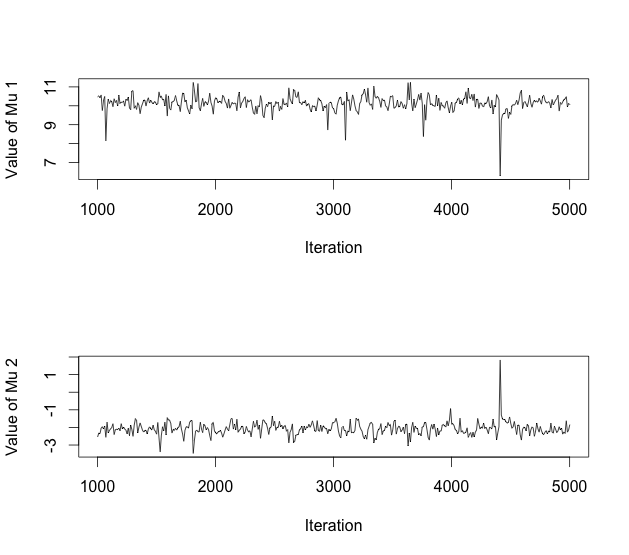
\includegraphics[width=\textwidth]{new-mu1.png}
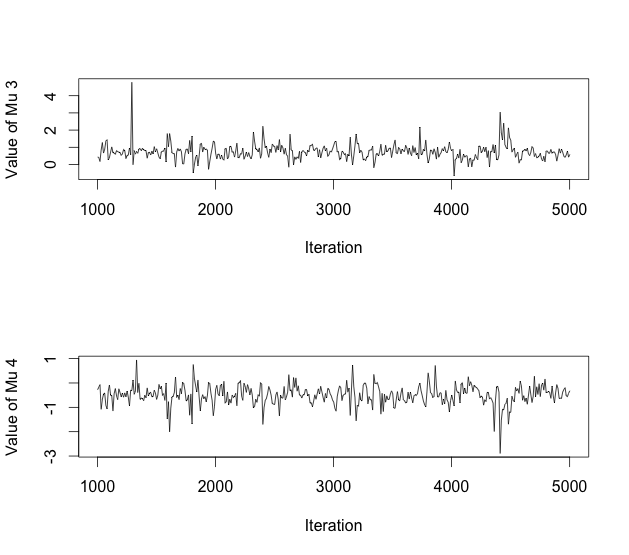
\includegraphics[width=\textwidth]{new-mu2.png}
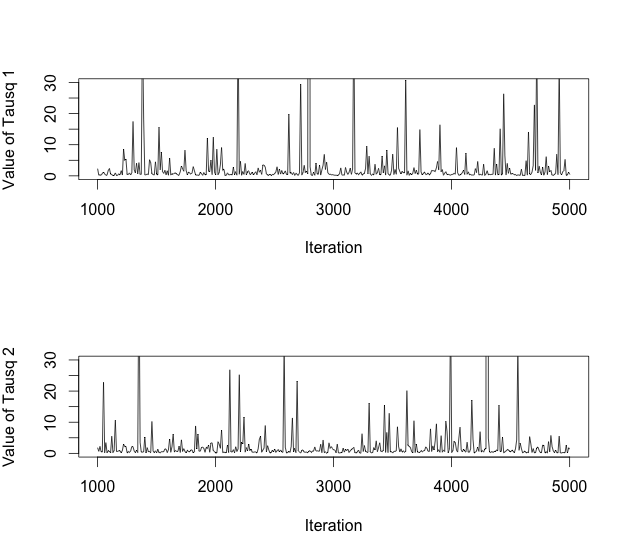
\includegraphics[width=\textwidth]{new-tau1.png}
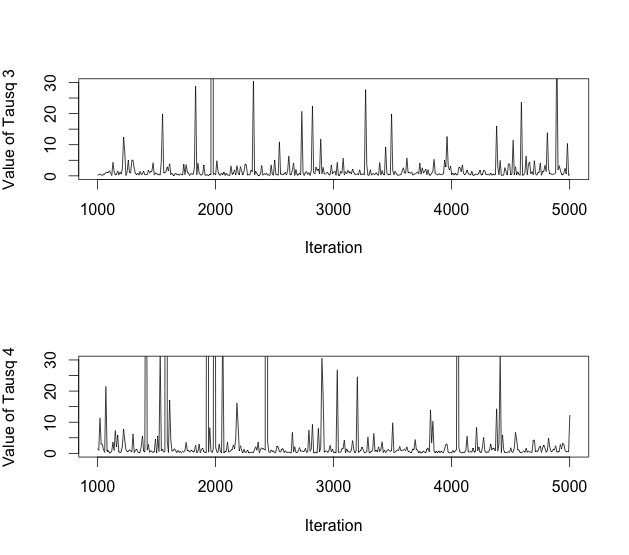
\includegraphics[width=\textwidth]{new-tau2.png}
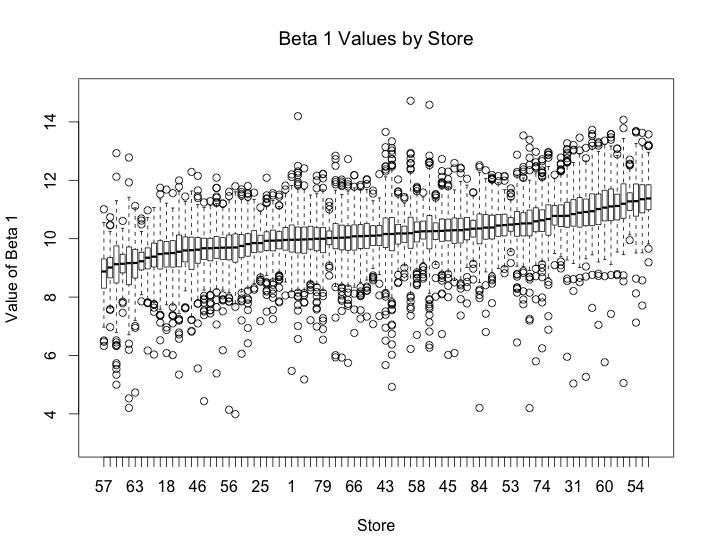
\includegraphics[height=12cm, keepaspectratio]{new-beta1.png}\\
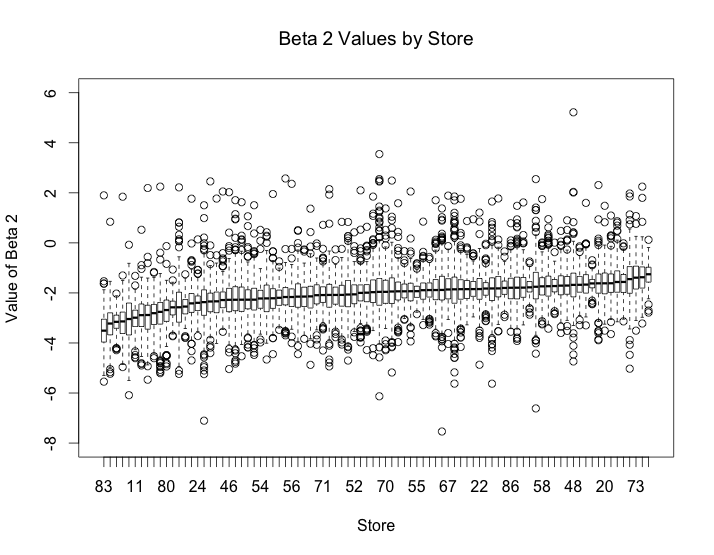
\includegraphics[height=12cm, keepaspectratio]{new-beta2.png}\\
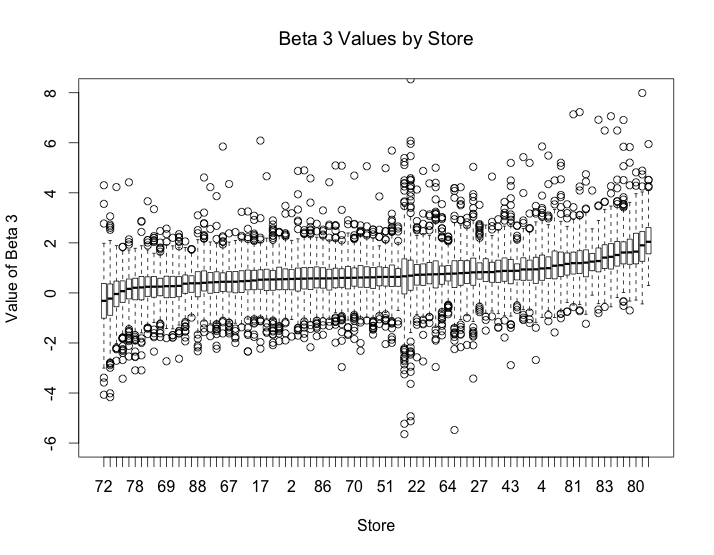
\includegraphics[height=12cm, keepaspectratio]{new-beta3.png}\\
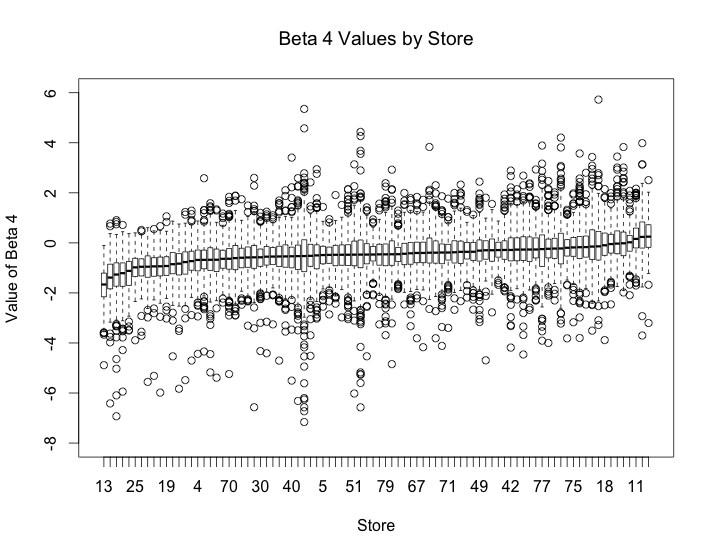
\includegraphics[height=12cm, keepaspectratio]{new-beta4.png}\\

\subsection{Full R Code}
\begin{knitrout}
\definecolor{shadecolor}{rgb}{0.969, 0.969, 0.969}\color{fgcolor}\begin{kframe}
\begin{alltt}
\hlcom{# StatMod2 - Cheese - Basic Hierarchical Model Version}

\hlkwd{library}\hlstd{(reshape)}
\hlkwd{library}\hlstd{(ggplot2)}

\hlcom{# Fetch and prepare data.}
\hlstd{path} \hlkwb{<-} \hlkwd{paste}\hlstd{(}\hlstr{"~/Google Drive/2. SPRING 2015/STAT MOD 2 - Prof Scott/"}\hlstd{,}
              \hlstr{"hierarch-shrinkage/cheese"}\hlstd{,} \hlkwc{sep}\hlstd{=}\hlstr{""}\hlstd{)}
\hlkwd{setwd}\hlstd{(path)}
\hlstd{data} \hlkwb{<-} \hlkwd{read.csv}\hlstd{(}\hlstr{"cheese.csv"}\hlstd{)}
\hlstd{data}\hlopt{$}\hlstd{log.Q} \hlkwb{<-} \hlkwd{log}\hlstd{(data}\hlopt{$}\hlstd{vol)}
\hlstd{data}\hlopt{$}\hlstd{log.P} \hlkwb{<-} \hlkwd{log}\hlstd{(data}\hlopt{$}\hlstd{price)}
\hlstd{data}\hlopt{$}\hlstd{cross} \hlkwb{<-} \hlstd{data}\hlopt{$}\hlstd{log.P}\hlopt{*}\hlstd{data}\hlopt{$}\hlstd{disp}
\hlstd{data} \hlkwb{<-} \hlstd{data[,}\hlkwd{c}\hlstd{(}\hlnum{1}\hlstd{,} \hlnum{5}\hlstd{,} \hlnum{6}\hlstd{,} \hlnum{4}\hlstd{,} \hlnum{7}\hlstd{)]}
\hlstd{data} \hlkwb{<-} \hlstd{data[}\hlkwd{order}\hlstd{(data[,}\hlnum{1}\hlstd{]),]}
\hlkwd{attach}\hlstd{(data)}

\hlstd{sigma2} \hlkwb{<-} \hlnum{1}\hlopt{/}\hlkwd{rgamma}\hlstd{(}\hlnum{1}\hlstd{,} \hlnum{0.5}\hlstd{,} \hlnum{0.5}\hlstd{)}
\hlstd{a0}\hlkwb{=}\hlnum{0.5}\hlstd{; b0}\hlkwb{=}\hlnum{0.5}\hlstd{;} \hlcom{# Hyper params for Tau's, which are ~ InvGamma.}
\hlstd{a1}\hlkwb{=}\hlnum{0.5}\hlstd{; b1}\hlkwb{=}\hlnum{0.5}\hlstd{;}
\hlstd{a2}\hlkwb{=}\hlnum{0.5}\hlstd{; b2}\hlkwb{=}\hlnum{0.5}\hlstd{;}
\hlstd{a3}\hlkwb{=}\hlnum{0.5}\hlstd{; b3}\hlkwb{=}\hlnum{0.5}\hlstd{;}
\hlstd{m0}\hlkwb{=}\hlnum{10}\hlstd{; v0}\hlkwb{=}\hlnum{1000}\hlstd{;} \hlcom{# Hyper params for Mu's, which are ~ Normal.}
\hlstd{m1}\hlkwb{=}\hlopt{-}\hlnum{1}\hlstd{; v1}\hlkwb{=}\hlnum{1000}\hlstd{;}
\hlstd{m2}\hlkwb{=}\hlnum{1}\hlstd{; v2}\hlkwb{=}\hlnum{1000}\hlstd{;}
\hlstd{m3}\hlkwb{=}\hlopt{-}\hlnum{1}\hlstd{; v3}\hlkwb{=}\hlnum{1000}\hlstd{;}

\hlstd{Gibbs} \hlkwb{<-} \hlkwa{function}\hlstd{(}\hlkwc{data}\hlstd{) \{}
  \hlstd{t0sq} \hlkwb{<-} \hlnum{1}\hlopt{/}\hlkwd{rgamma}\hlstd{(}\hlnum{1}\hlstd{, a0, b0)} \hlcom{# Initialize Tau's.}
  \hlstd{t1sq} \hlkwb{<-} \hlnum{1}\hlopt{/}\hlkwd{rgamma}\hlstd{(}\hlnum{1}\hlstd{, a1, b1)}
  \hlstd{t2sq} \hlkwb{<-} \hlnum{1}\hlopt{/}\hlkwd{rgamma}\hlstd{(}\hlnum{1}\hlstd{, a2, b2)}
  \hlstd{t3sq} \hlkwb{<-} \hlnum{1}\hlopt{/}\hlkwd{rgamma}\hlstd{(}\hlnum{1}\hlstd{, a3, b3)}
  \hlstd{mu0} \hlkwb{<-} \hlkwd{rnorm}\hlstd{(}\hlnum{1}\hlstd{, m0, v0)} \hlcom{# Initialize Mu's.}
  \hlstd{mu1} \hlkwb{<-} \hlkwd{rnorm}\hlstd{(}\hlnum{1}\hlstd{, m1, v1)}
  \hlstd{mu2} \hlkwb{<-} \hlkwd{rnorm}\hlstd{(}\hlnum{1}\hlstd{, m2, v2)}
  \hlstd{mu3} \hlkwb{<-} \hlkwd{rnorm}\hlstd{(}\hlnum{1}\hlstd{, m3, v3)}
  \hlstd{n.iter} \hlkwb{<-} \hlnum{2000}

  \hlcom{# Prepare per-store data.}
  \hlstd{store.names} \hlkwb{<-} \hlkwd{unique}\hlstd{(data}\hlopt{$}\hlstd{store)}
  \hlstd{num.stores} \hlkwb{<-} \hlkwd{length}\hlstd{(store.names)}

  \hlcom{# Create containers for chains and variables.}
  \hlstd{PARAMS.BY.STORE} \hlkwb{<-} \hlkwd{array}\hlstd{(}\hlkwd{rep}\hlstd{(}\hlnum{NA}\hlstd{, num.stores}\hlopt{*}\hlnum{4}\hlopt{*}\hlstd{n.iter),}
                           \hlkwd{c}\hlstd{(num.stores,} \hlnum{4}\hlstd{, n.iter))}
  \hlstd{MU} \hlkwb{<-} \hlkwd{matrix}\hlstd{(}\hlnum{NA}\hlstd{,} \hlkwc{nrow}\hlstd{=n.iter}\hlopt{+}\hlnum{1}\hlstd{,} \hlkwc{ncol}\hlstd{=}\hlnum{4}\hlstd{)}
  \hlstd{MU[}\hlnum{1}\hlstd{,]} \hlkwb{<-} \hlkwd{c}\hlstd{(mu0, mu1, mu2, mu3)}
  \hlstd{TAUSQ} \hlkwb{<-} \hlkwd{matrix}\hlstd{(}\hlnum{NA}\hlstd{,} \hlkwc{nrow}\hlstd{=n.iter}\hlopt{+}\hlnum{1}\hlstd{,} \hlkwc{ncol}\hlstd{=}\hlnum{4}\hlstd{)}
  \hlstd{TAUSQ[}\hlnum{1}\hlstd{,]} \hlkwb{<-} \hlkwd{c}\hlstd{(t0sq, t1sq, t2sq, t3sq)}

  \hlcom{# Do Gibbs many times.}

  \hlkwa{for} \hlstd{(iter} \hlkwa{in} \hlnum{1}\hlopt{:}\hlstd{n.iter) \{}

    \hlcom{# Sample Beta's (be0, be1, be2, be3) for each store.}
    \hlcom{# Use Normal-Normal full conditional posterior.}
    \hlkwa{for} \hlstd{(i} \hlkwa{in} \hlnum{1}\hlopt{:}\hlstd{num.stores) \{}
      \hlstd{name} \hlkwb{<-} \hlkwd{toString}\hlstd{(store.names[i])}
      \hlstd{store.data} \hlkwb{<-} \hlstd{data[}\hlkwd{which}\hlstd{(data}\hlopt{$}\hlstd{store}\hlopt{==}\hlstd{name),]}
      \hlstd{ni} \hlkwb{<-} \hlkwd{dim}\hlstd{(store.data)[}\hlnum{1}\hlstd{]}
      \hlstd{y} \hlkwb{<-} \hlstd{store.data}\hlopt{$}\hlstd{log.Q}
      \hlstd{X} \hlkwb{<-} \hlkwd{as.matrix}\hlstd{(}\hlkwd{cbind}\hlstd{(}\hlkwd{rep}\hlstd{(}\hlnum{1}\hlstd{, ni),}
                           \hlstd{store.data[,}\hlkwd{c}\hlstd{(}\hlstr{"log.P"}\hlstd{,} \hlstr{"disp"}\hlstd{,} \hlstr{"cross"}\hlstd{)]))}
      \hlstd{XtX} \hlkwb{<-} \hlkwd{t}\hlstd{(X)}\hlopt\hlstd{X}
      \hlstd{Xty} \hlkwb{<-} \hlkwd{t}\hlstd{(X)}\hlopt\hlstd{y}
      \hlstd{latest.mu} \hlkwb{<-} \hlstd{MU[iter,]}
      \hlstd{diag.tausqs} \hlkwb{<-} \hlkwd{diag}\hlstd{(}\hlkwd{c}\hlstd{(t0sq, t1sq, t2sq, t3sq))}
      \hlstd{b} \hlkwb{<-} \hlkwd{sample.beta}\hlstd{(sigma2, diag.tausqs, XtX, Xty, latest.mu)}
      \hlstd{PARAMS.BY.STORE[i,,iter]} \hlkwb{<-} \hlstd{b}
    \hlstd{\}}

    \hlcom{# Use Normal-Normal full conditional posterior to update Mu's, given Beta's.}
    \hlstd{beta.means} \hlkwb{<-} \hlkwd{colMeans}\hlstd{(PARAMS.BY.STORE[,,iter])}
    \hlstd{mu0} \hlkwb{<-} \hlkwd{sample.mu}\hlstd{(m0, v0, num.stores, beta.means[}\hlnum{1}\hlstd{], t0sq)}
    \hlstd{mu1} \hlkwb{<-} \hlkwd{sample.mu}\hlstd{(m1, v1, num.stores, beta.means[}\hlnum{2}\hlstd{], t1sq)}
    \hlstd{mu2} \hlkwb{<-} \hlkwd{sample.mu}\hlstd{(m2, v2, num.stores, beta.means[}\hlnum{3}\hlstd{], t2sq)}
    \hlstd{mu3} \hlkwb{<-} \hlkwd{sample.mu}\hlstd{(m3, v3, num.stores, beta.means[}\hlnum{4}\hlstd{], t3sq)}
    \hlstd{MU[iter}\hlopt{+}\hlnum{1}\hlstd{,]} \hlkwb{<-} \hlkwd{c}\hlstd{(mu0, mu1, mu2, mu3)}

    \hlcom{# Use Normal-InvGamma full conditional posterior to update Tau's, given Beta's.}
    \hlstd{t0sq} \hlkwb{<-} \hlkwd{sample.tausq}\hlstd{(beta.means[}\hlnum{1}\hlstd{], MU[iter,][}\hlnum{1}\hlstd{], a0, b0)}
    \hlstd{t1sq} \hlkwb{<-} \hlkwd{sample.tausq}\hlstd{(beta.means[}\hlnum{2}\hlstd{], MU[iter,][}\hlnum{2}\hlstd{], a1, b1)}
    \hlstd{t2sq} \hlkwb{<-} \hlkwd{sample.tausq}\hlstd{(beta.means[}\hlnum{3}\hlstd{], MU[iter,][}\hlnum{3}\hlstd{], a2, b2)}
    \hlstd{t3sq} \hlkwb{<-} \hlkwd{sample.tausq}\hlstd{(beta.means[}\hlnum{4}\hlstd{], MU[iter,][}\hlnum{4}\hlstd{], a3, b3)}
    \hlstd{TAUSQ[iter}\hlopt{+}\hlnum{1}\hlstd{,]} \hlkwb{<-} \hlkwd{c}\hlstd{(t0sq, t1sq, t2sq, t3sq)}
  \hlstd{\}}

  \hlkwd{return} \hlstd{(}\hlkwd{list}\hlstd{(}\hlkwc{PARAMS.BY.STORE}\hlstd{=PARAMS.BY.STORE,} \hlkwc{MU}\hlstd{=MU,} \hlkwc{TAUSQ}\hlstd{=TAUSQ))}
\hlstd{\}}

\hlstd{sample.beta} \hlkwb{<-} \hlkwa{function}\hlstd{(}\hlkwc{sigma2}\hlstd{,} \hlkwc{diag.tausqs}\hlstd{,} \hlkwc{XtX}\hlstd{,} \hlkwc{Xty}\hlstd{,} \hlkwc{latest.mu}\hlstd{) \{}
  \hlstd{cov} \hlkwb{<-} \hlkwd{ginv}\hlstd{(XtX}\hlopt{/}\hlstd{sigma2} \hlopt{+} \hlkwd{solve}\hlstd{(diag.tausqs))}
  \hlstd{mean} \hlkwb{<-} \hlstd{cov}\hlopt\hlstd{(Xty}\hlopt{/}\hlstd{sigma2} \hlopt{+} \hlkwd{solve}\hlstd{(diag.tausqs)}\hlopt\hlstd{latest.mu)}
  \hlstd{beta} \hlkwb{<-} \hlkwd{mvrnorm}\hlstd{(}\hlnum{1}\hlstd{,} \hlkwc{mu}\hlstd{=mean,} \hlkwc{Sigma}\hlstd{=cov)}
  \hlkwd{return} \hlstd{(beta)}
\hlstd{\}}
\hlstd{sample.mu} \hlkwb{<-} \hlkwa{function}\hlstd{(}\hlkwc{mu.pr.mean}\hlstd{,} \hlkwc{mu.pr.var}\hlstd{,} \hlkwc{num.stores}\hlstd{,} \hlkwc{beta.mean}\hlstd{,} \hlkwc{beta.var}\hlstd{) \{}
  \hlstd{var} \hlkwb{<-} \hlkwd{ginv}\hlstd{(}\hlnum{1}\hlopt{/}\hlstd{mu.pr.var} \hlopt{+} \hlstd{num.stores}\hlopt{/}\hlstd{beta.var)}
  \hlstd{mean} \hlkwb{<-} \hlstd{var}\hlopt{*}\hlstd{(mu.pr.mean}\hlopt{/}\hlstd{mu.pr.var} \hlopt{+} \hlstd{num.stores}\hlopt{*}\hlstd{beta.mean}\hlopt{/}\hlstd{beta.var)}
  \hlstd{mu0} \hlkwb{<-} \hlkwd{rnorm}\hlstd{(}\hlnum{1}\hlstd{,} \hlkwc{mean}\hlstd{=mean,} \hlkwc{sd}\hlstd{=}\hlkwd{sqrt}\hlstd{(var))}
  \hlkwd{return} \hlstd{(mu0)}
\hlstd{\}}
\hlstd{sample.tausq} \hlkwb{<-} \hlkwa{function}\hlstd{(}\hlkwc{be0}\hlstd{,} \hlkwc{mu0}\hlstd{,} \hlkwc{pr.a}\hlstd{,} \hlkwc{pr.b}\hlstd{) \{}
  \hlstd{shape} \hlkwb{<-} \hlstd{pr.a} \hlopt{+} \hlnum{1}\hlopt{/}\hlnum{2}
  \hlstd{rate} \hlkwb{<-} \hlnum{1}\hlopt{/}\hlnum{2}\hlopt{*}\hlstd{(be0}\hlopt{-}\hlstd{mu0)}\hlopt{^}\hlnum{2} \hlopt{+} \hlstd{pr.b}
  \hlstd{tausq} \hlkwb{<-} \hlkwd{rgamma}\hlstd{(}\hlnum{1}\hlstd{,} \hlkwc{shape}\hlstd{=shape,} \hlkwc{rate}\hlstd{=rate)}
  \hlkwd{return} \hlstd{(}\hlnum{1}\hlopt{/}\hlstd{tausq)}
\hlstd{\}}

\hlstd{results} \hlkwb{<-} \hlkwd{Gibbs}\hlstd{(data)}
\hlstd{P} \hlkwb{<-} \hlstd{results}\hlopt{$}\hlstd{PARAMS.BY.STORE}
\hlstd{MU} \hlkwb{<-} \hlstd{results}\hlopt{$}\hlstd{MU}
\hlstd{TAUSQ} \hlkwb{<-} \hlstd{results}\hlopt{$}\hlstd{TAUSQ}

\hlcom{# Show traceplots for Mu's and Tau's.}
\hlkwd{par}\hlstd{(}\hlkwc{mfrow}\hlstd{=}\hlkwd{c}\hlstd{(}\hlnum{2}\hlstd{,} \hlnum{2}\hlstd{))}
\hlstd{its} \hlkwb{<-} \hlnum{1}\hlopt{:}\hlkwd{dim}\hlstd{(MU)[}\hlnum{1}\hlstd{]}
\hlstd{its} \hlkwb{<-} \hlstd{its[}\hlkwd{seq}\hlstd{(}\hlnum{1001}\hlstd{,} \hlkwd{dim}\hlstd{(MU)[}\hlnum{1}\hlstd{],} \hlnum{10}\hlstd{)]}
\hlstd{count} \hlkwb{<-} \hlkwd{dim}\hlstd{(MU)[}\hlnum{2}\hlstd{]}
\hlkwa{for} \hlstd{(p} \hlkwa{in} \hlnum{1}\hlopt{:}\hlstd{count) \{}
  \hlkwd{plot}\hlstd{(its, MU[,p][}\hlkwd{seq}\hlstd{(}\hlnum{1001}\hlstd{,} \hlkwd{dim}\hlstd{(MU)[}\hlnum{1}\hlstd{],} \hlnum{10}\hlstd{)],} \hlkwc{xlab}\hlstd{=}\hlstr{"Iteration"}\hlstd{,}
       \hlkwc{ylab}\hlstd{=}\hlkwd{bquote}\hlstd{(}\hlstr{"Value of Mu"}\hlopt{~}\hlkwd{.}\hlstd{(p)),} \hlkwc{type}\hlstd{=}\hlstr{"l"}\hlstd{)}
\hlstd{\}}
\hlkwa{for} \hlstd{(p} \hlkwa{in} \hlnum{1}\hlopt{:}\hlstd{count) \{}
  \hlkwd{plot}\hlstd{(its, TAUSQ[,p][}\hlkwd{seq}\hlstd{(}\hlnum{1001}\hlstd{,} \hlkwd{dim}\hlstd{(MU)[}\hlnum{1}\hlstd{],} \hlnum{10}\hlstd{)],} \hlkwc{xlab}\hlstd{=}\hlstr{"Iteration"}\hlstd{,}
       \hlkwc{ylab}\hlstd{=}\hlkwd{bquote}\hlstd{(}\hlstr{"Value of Tausq"}\hlopt{~}\hlkwd{.}\hlstd{(p)),} \hlkwc{type}\hlstd{=}\hlstr{"l"}\hlstd{,}
       \hlkwc{ylim}\hlstd{=}\hlkwd{c}\hlstd{(}\hlnum{0}\hlstd{,} \hlnum{30}\hlstd{))}
\hlstd{\}}

\hlcom{# Show boxplots for betas of all stores together.}
\hlkwd{par}\hlstd{(}\hlkwc{mfrow}\hlstd{=}\hlkwd{c}\hlstd{(}\hlnum{2}\hlstd{,}\hlnum{2}\hlstd{))}
\hlkwa{for} \hlstd{(p} \hlkwa{in} \hlnum{1}\hlopt{:}\hlstd{count) \{}
  \hlstd{data.to.plot} \hlkwb{<-} \hlkwd{t}\hlstd{(P[,p,}\hlkwd{seq}\hlstd{(}\hlnum{1001}\hlstd{,} \hlkwd{dim}\hlstd{(MU)[}\hlnum{1}\hlstd{]}\hlopt{-}\hlnum{1}\hlstd{,} \hlnum{10}\hlstd{)])}
  \hlstd{m} \hlkwb{<-} \hlkwd{melt}\hlstd{(data.to.plot)[}\hlkwd{c}\hlstd{(}\hlnum{2}\hlstd{,} \hlnum{3}\hlstd{)]}
  \hlkwd{names}\hlstd{(m)} \hlkwb{<-} \hlkwd{c}\hlstd{(}\hlstr{"store"}\hlstd{,} \hlstr{"value"}\hlstd{)}
  \hlstd{bymedian} \hlkwb{<-} \hlkwd{with}\hlstd{(m,} \hlkwd{reorder}\hlstd{(m}\hlopt{$}\hlstd{store, m}\hlopt{$}\hlstd{value, median))}
  \hlkwd{boxplot}\hlstd{(m}\hlopt{$}\hlstd{value} \hlopt{~} \hlstd{bymedian,} \hlkwc{data}\hlstd{=m,} \hlkwc{xlab}\hlstd{=}\hlstr{"Store"}\hlstd{,}
          \hlkwc{ylab}\hlstd{=}\hlkwd{bquote}\hlstd{(}\hlstr{"Value of Beta"}\hlopt{~}\hlkwd{.}\hlstd{(p)),}
          \hlkwc{main}\hlstd{=}\hlkwd{bquote}\hlstd{(}\hlstr{"Beta"}\hlopt{~}\hlkwd{.}\hlstd{(p)}\hlopt{~}\hlstr{"Values by Store"}\hlstd{),}
          \hlkwc{ylim}\hlstd{=}\hlkwd{c}\hlstd{(}\hlnum{3}\hlstd{,}\hlnum{15}\hlstd{))}
\hlstd{\}}
\end{alltt}
\end{kframe}
\end{knitrout}

\end{document}


